% !TEX program = pdflatex
\documentclass[handout]{beamer}
% \documentclass{beamer}

\usetheme{Madrid}
\usecolortheme{default}

\definecolor{THUpurple}{RGB}{102,8,116}

\usepackage{caption}
\usepackage{listings}
\usepackage{xcolor}
\lstset{language=Python,keywordstyle={\bfseries \color{blue}}}
\usepackage{pdfpages}
\usepackage{makecell}

\newcommand{\ud}{\mathrm{d}}
\newcommand{\mev}{\mathrm{MeV}}
\newcommand{\gev}{\mathrm{GeV}}

\setbeamercolor{structure}{fg=THUpurple}
\setbeamersize{text margin left=10mm,text margin right=10mm}
% \setlength{\belowcaptionskip}{-2mm}
\title[Waveform Analysis]{A Comprehensive Survey of PMT Waveform Analysis Methods}
% \author[Dacheng Xu]{Dacheng Xu \\ [4mm] 
\includegraphics[height=1.5cm]{img/Tsinghua_University_Logo.png} \hspace{2mm} 
\includegraphics[height=1.5cm]{img/Js.png}}
% \institute[THU]{Tsinghua University \\ [2mm] On Behalf of \normalsize{Jinping Neutrino Experiment Collaboration}}
\date[DANCE]{July 28, 2020}
% \logo{
\includegraphics[height=1.5cm]{img/J.png}}

\AtBeginSection[]
{
    \begin{frame}
        \frametitle{Outline}
        \tableofcontents[currentsection]
    \end{frame}
}

\begin{document}
\captionsetup[figure]{labelfont={bf},name={Fig}}
\frame{\titlepage}

\begin{frame}
\frametitle{Outline}
\tableofcontents
\end{frame}

\section{Jinping Neutrino Experiment}
\begin{frame}
\frametitle{CJPL}
\begin{figure}
    \centering
    \caption{China JinPing Underground Laboratory}
    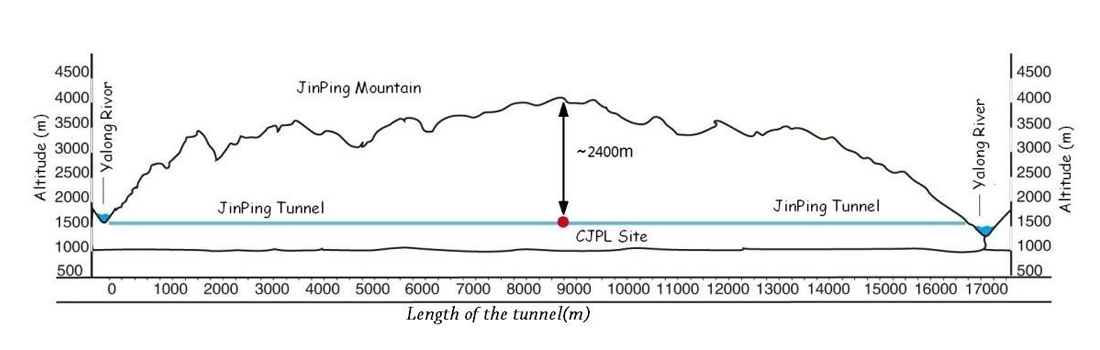
\includegraphics[width=1.0\linewidth]{img/mountain.png}
\end{figure}
\begin{itemize}
    \item Overburden $\sim2400\mathrm{m}$
    \item Extremely low cosmic-ray $\mu$ flux
    \item Low reactor neutrino flux
    \item Ideal site of low background neutrino physics research
\end{itemize}
\end{frame}

\begin{frame}
\frametitle{Jinping Neutrino Experiment}
\setlength{\abovecaptionskip}{-2mm}
\begin{figure}
    \centering
    
\includegraphics[width=0.3\linewidth]{img/J.png}
\end{figure}
\vspace{-4mm}
\begin{columns}
\column{0.5\textwidth}
\begin{center}
    Ongoing
\end{center}
\begin{figure}
    \centering
    \caption{1-ton prototype}
    \includegraphics[width=0.6\linewidth]{img/prototype.jpeg}
\end{figure}
\column{0.5\textwidth}
\begin{center}
    Futuristic
\end{center}
\begin{figure}
    \centering
    \caption{$\sim$100t detector}
    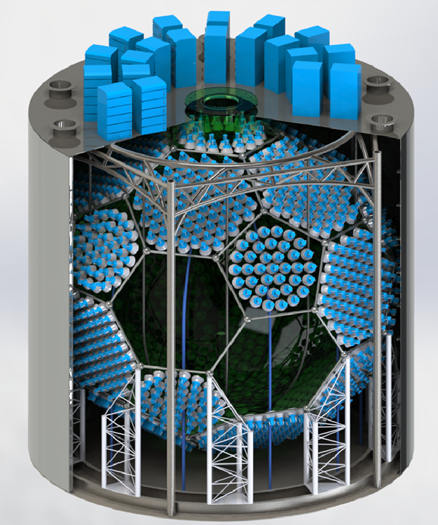
\includegraphics[width=0.6\linewidth]{img/100tondetector.png}
\end{figure}
\end{columns}
\end{frame}

\section{Motivation}
\begin{frame}
\frametitle{Photomultiplier Tube}
\setlength{\abovecaptionskip}{0mm}
\setlength{\belowcaptionskip}{0mm}
\begin{columns}
\column{0.6\textwidth}
\begin{figure}
    \centering
    \caption{PMT}
    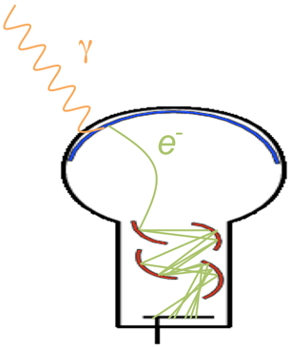
\includegraphics[width=0.3\linewidth]{img/PMT.png}
\end{figure}
\begin{figure}
    \centering
    \caption{PMT Single PE response}
    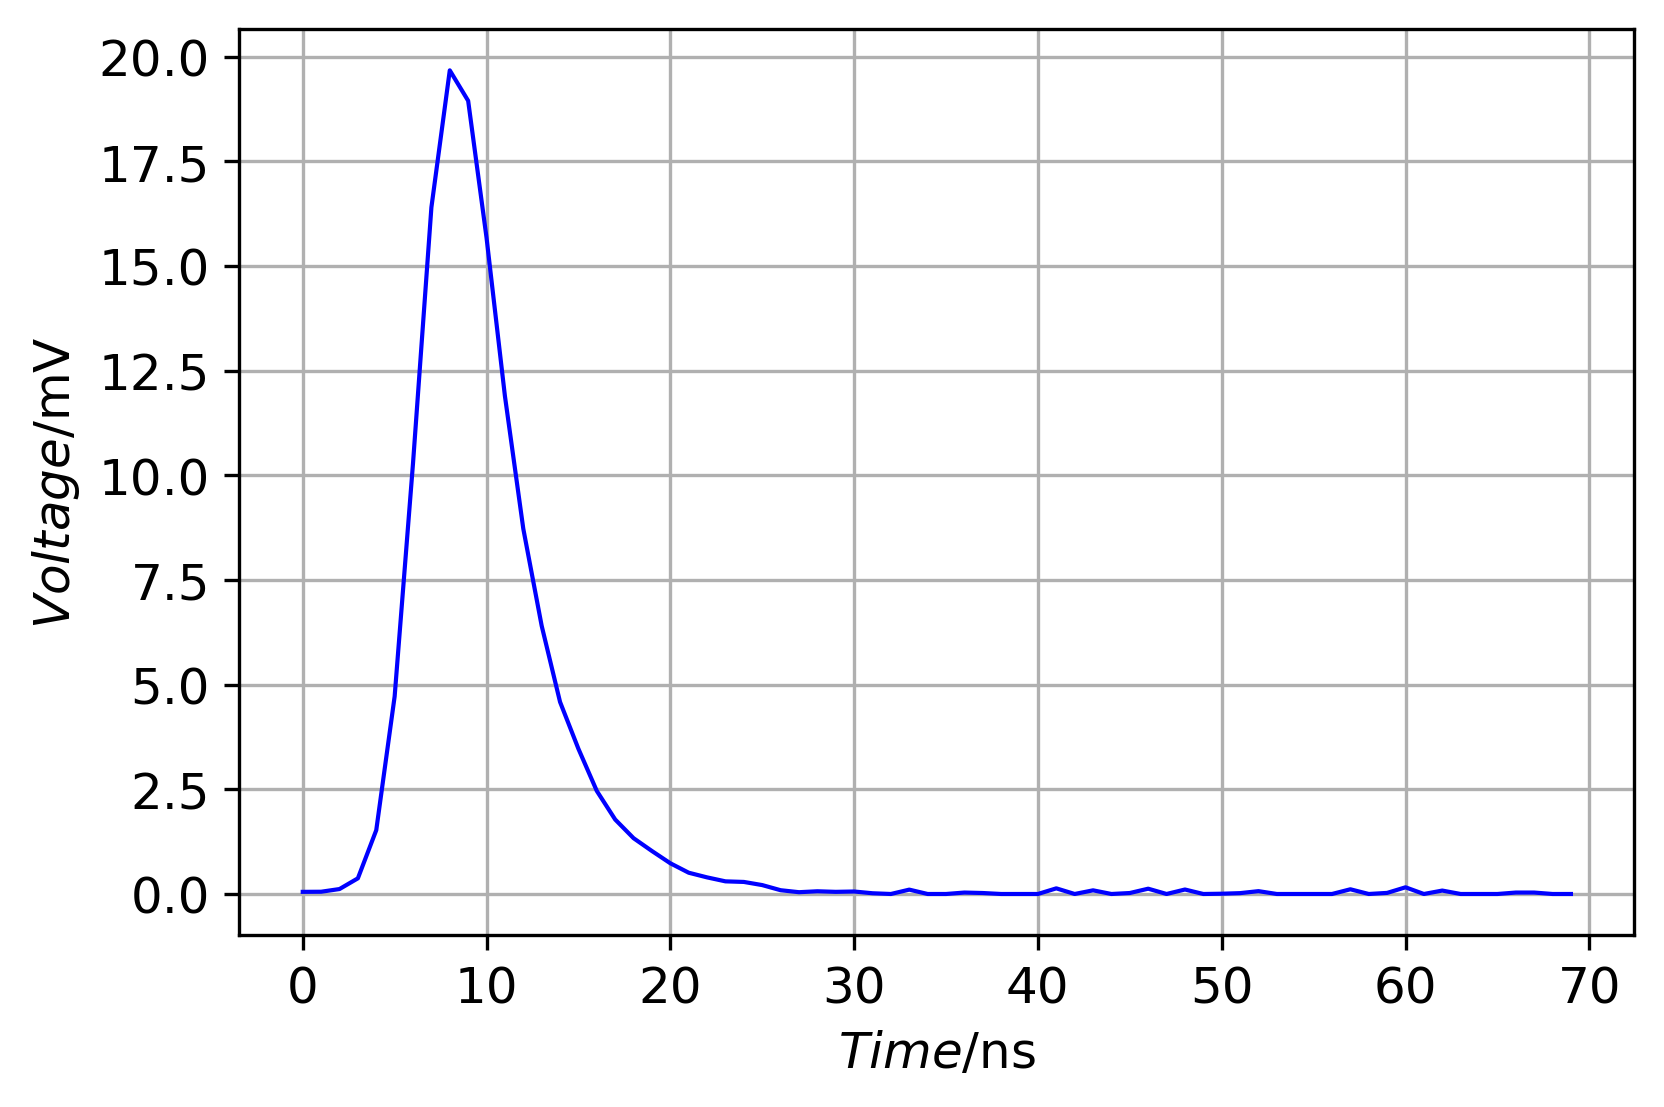
\includegraphics[width=0.9\linewidth]{img/pmtspe.png}
\end{figure}
\column{0.4\textwidth}
\begin{center}
    3 individual processes:
\end{center}
\begin{itemize}
    \item Photon detection
    \item Photon-Electron conversion
    \item Electron collection
\end{itemize}
\end{columns}
\end{frame}

\begin{frame}
\frametitle{Previous Method}
\hspace{4mm}Previously, when handling PMT waveforms, we record:
\begin{itemize}
    \item First HitTime
    \item Integration of Waveform(Charge)
\end{itemize}
\begin{figure}
    \centering
    % \caption{Traditional Recorded Waveform}
    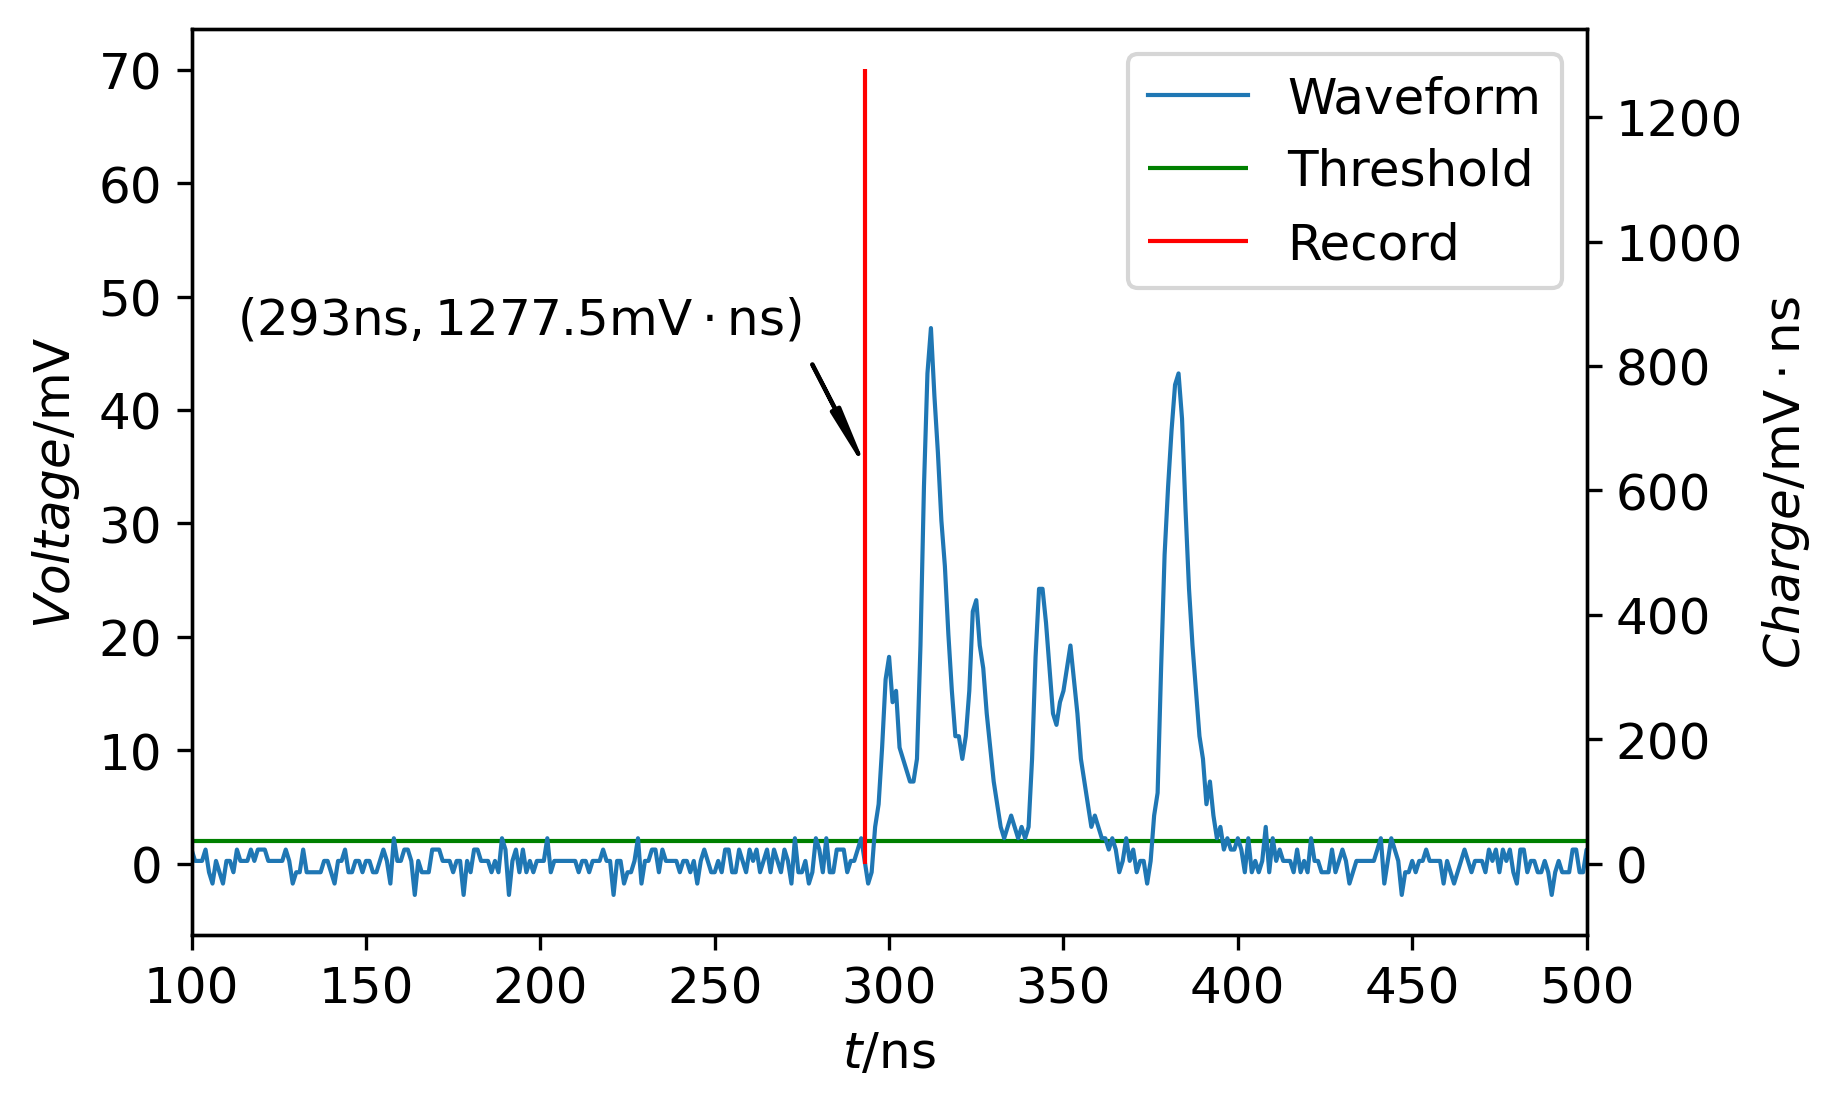
\includegraphics[width=0.8\linewidth]{img/previous.png}
\end{figure}
\end{frame}

\begin{frame}
\frametitle{New Goal}
\begin{itemize}
    \item Extract All Detailed Photon Information in 1 Window
    \item Including: RiseTime (The time when electron hit first dynode) \& Charge or PEnumber
\end{itemize}
\begin{figure}
    \centering
    % \caption{Traditional Recorded Waveform}
    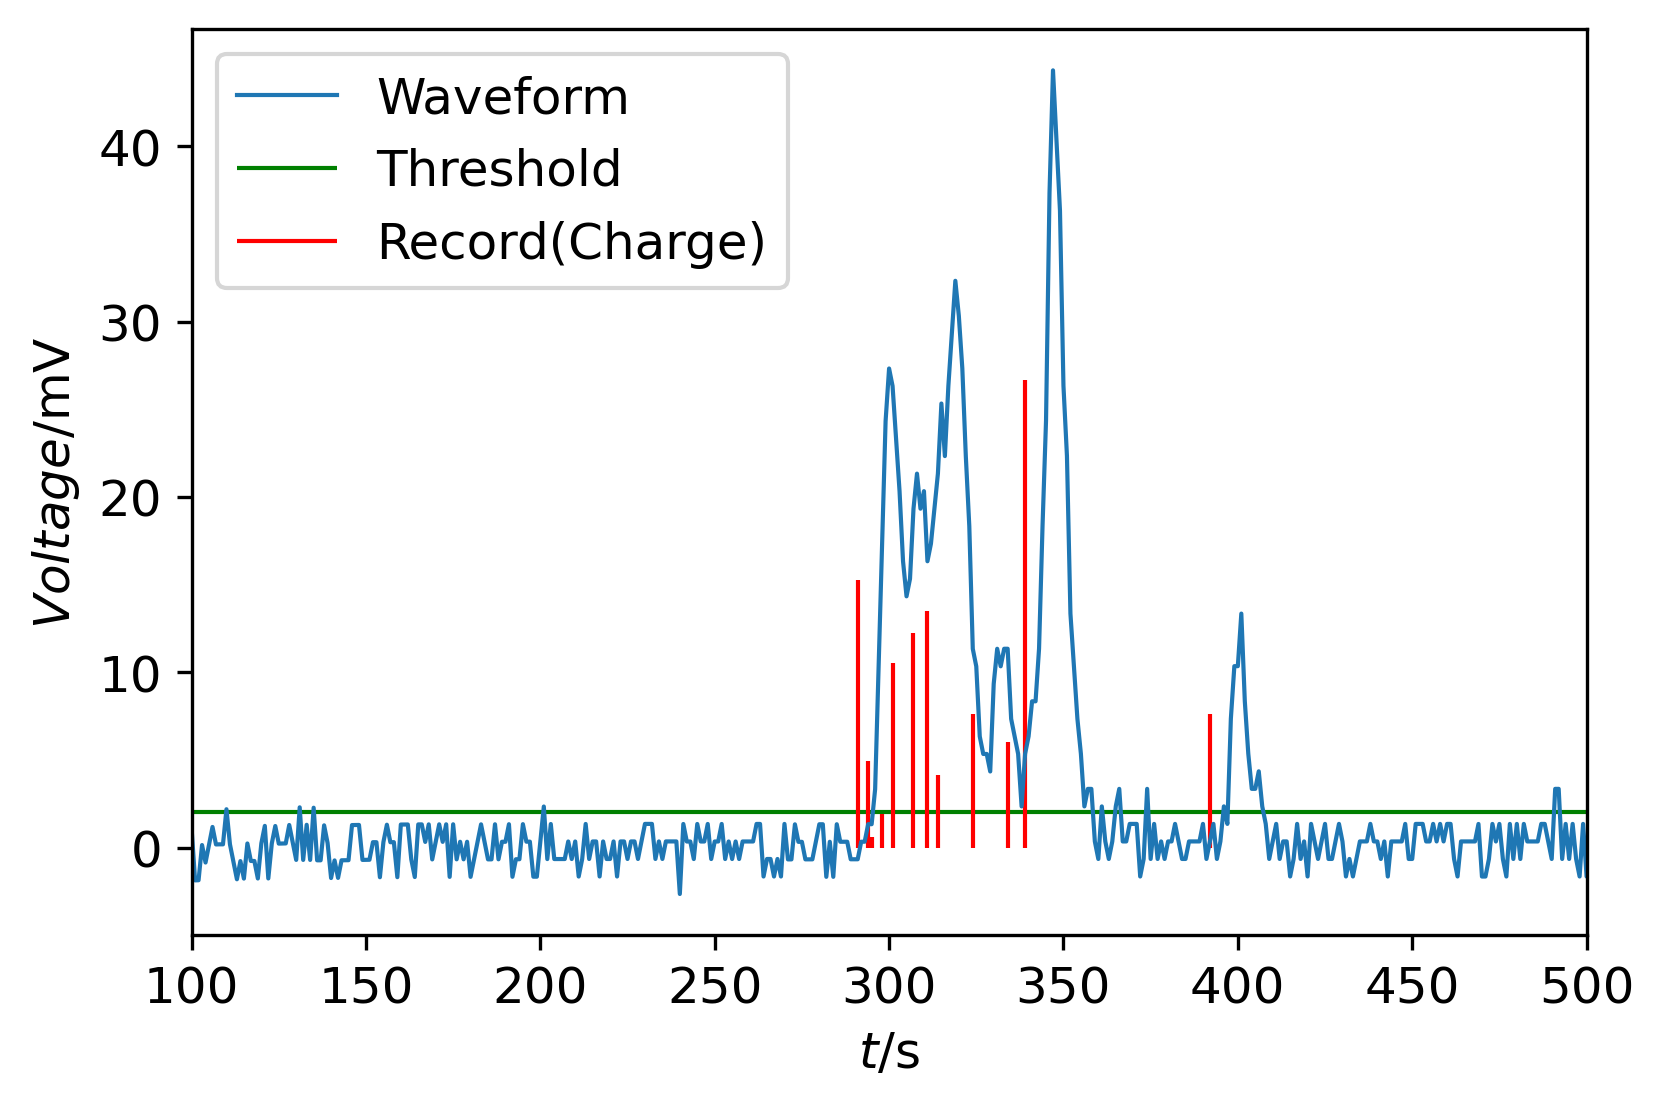
\includegraphics[width=0.8\linewidth]{img/goal.png}
\end{figure}
\end{frame}

\section{Wasserstein Distance \& Poisson Distance}
\begin{frame}
\frametitle{Measurement of difference}
\begin{center}
    The difference between Reconstruction Result \& Truth?
\end{center}
\end{frame}

\begin{frame}
\frametitle{Wasserstein Distance}
Let ($\chi$, $d$) be a Polish metric space, and let $p\in[1, +\infty)$. For any two probability measures $\mu, \nu$, on $\chi$, the Wasserstein distance of order $p$ between $\mu$ and $\nu$ is defined by formula\footnotemark[1]:
\begin{equation*}
    W_{p}(\mu, \nu) = (\inf_{\pi\in\Pi(\mu, \nu)} \int_{\chi}d(x, y)^{p}d\pi(x,y))^{1/p}
\end{equation*}
Which means: transporting mass with measure $\mu$ to have measure $\nu$ with minimal effort
\footnotetext[1]{Optimal transport: old and new, C{\'e}dric Villani, 2008}
\end{frame}

\begin{frame}
\frametitle{Wasserstein Distance}
In this work, we regard \textbf{normalised} Weight (Charge or PEnumber) as the discrete distribution (or probability mass function) of RiseTime, 
\begin{itemize}
    \item Which means: $Weight(RiseTime) = Pr(RiseTime)$
    \item Distance: $D_{w}=\sum_{i=0}^{1029}|CDF(RiseTime_{recon})_{i} - CDF(RiseTime_{truth})_{i}|$
    \item $CDF$: Cumulative distribution function, \\ PMT WindowSize = 1029$\mathrm{ns}$
    \item Example:\begin{itemize}
        \item $RiseTime_{recon} = [0, 1, 2, 3], Weight_{recon} = [0.3, 0.7, 0.0, 0.0]$, $RiseTime_{truth} = [0, 1, 2, 3], Weight_{truth} = [0.0, 0.0, 0.5, 0.5]$
        \item $CDF(RiseTime_{recon}) = [0.3, 1.0, 1.0, 1.0]$, \\ $CDF(RiseTime_{truth}) = [0.0, 0.0, 0.5, 1.0]$
        \item $D_{w} = SUM[Abs([0.3, 1.0, 1.0, 1.0] - [0.0, 0.0, 0.5, 1.0])] = 1.8$
        \end{itemize}
    \item It is proved that this definition of distance is equivalent to Wasserstein Distance (p=1)
\end{itemize}
\end{frame}

\begin{frame}
\frametitle{Poisson Distance}
\hspace{4mm}Poisson Distance is used \textbf{only} when reconstruct PEnumber
\begin{itemize}
    \item $Q = \sum_{i=0}^{1029}PEnumber_{truth_i}; q = \sum_{i=0}^{1029}PEnumber_{recon_i}$
    \item $D_{p} = |Q-q|*Poisson(Q|Q)$
\end{itemize}
\end{frame}

\section{Method of Convolutional Neural Network}

\begin{frame}
\frametitle{Input \& Output, Loss}
\hspace{4mm}Input \& Output:
\begin{itemize}
    \item Input: Pedestal deduced PMT waveform, length = 1029$\mathrm{ns}$
    \item Output: Weight (Charge or PEnumber) sequence, length = 1029$\mathrm{ns}$
\end{itemize}
\hspace{4mm}Loss function:
\begin{itemize}
    \item Wasserstein Distance \\ $D_{w}=\sum_{i=0}^{1029}|CDF(RiseTime_{recon})_{i} - CDF(RiseTime_{truth})_{i}|$
\end{itemize}
\end{frame}

\begin{frame}
\frametitle{Data Sample}
\begin{columns}
\column{0.5\textwidth}
\hspace{4mm}Dataset:
\begin{itemize}
    \item Events of $e^{-}$ within $1\mev$ to $8\mev$
\end{itemize}
\column{0.5\textwidth}
\begin{figure}
    \centering
    \caption{Data Structure}
    \includegraphics[width=1.0\linewidth]{img/dataset.png}
\end{figure}
\end{columns}
\end{frame}

\begin{frame}
\frametitle{CNN Structure}
\begin{columns}
\column{0.35\textwidth}
\begin{figure}[H]
    \centering
    \caption{CNN Structure}
    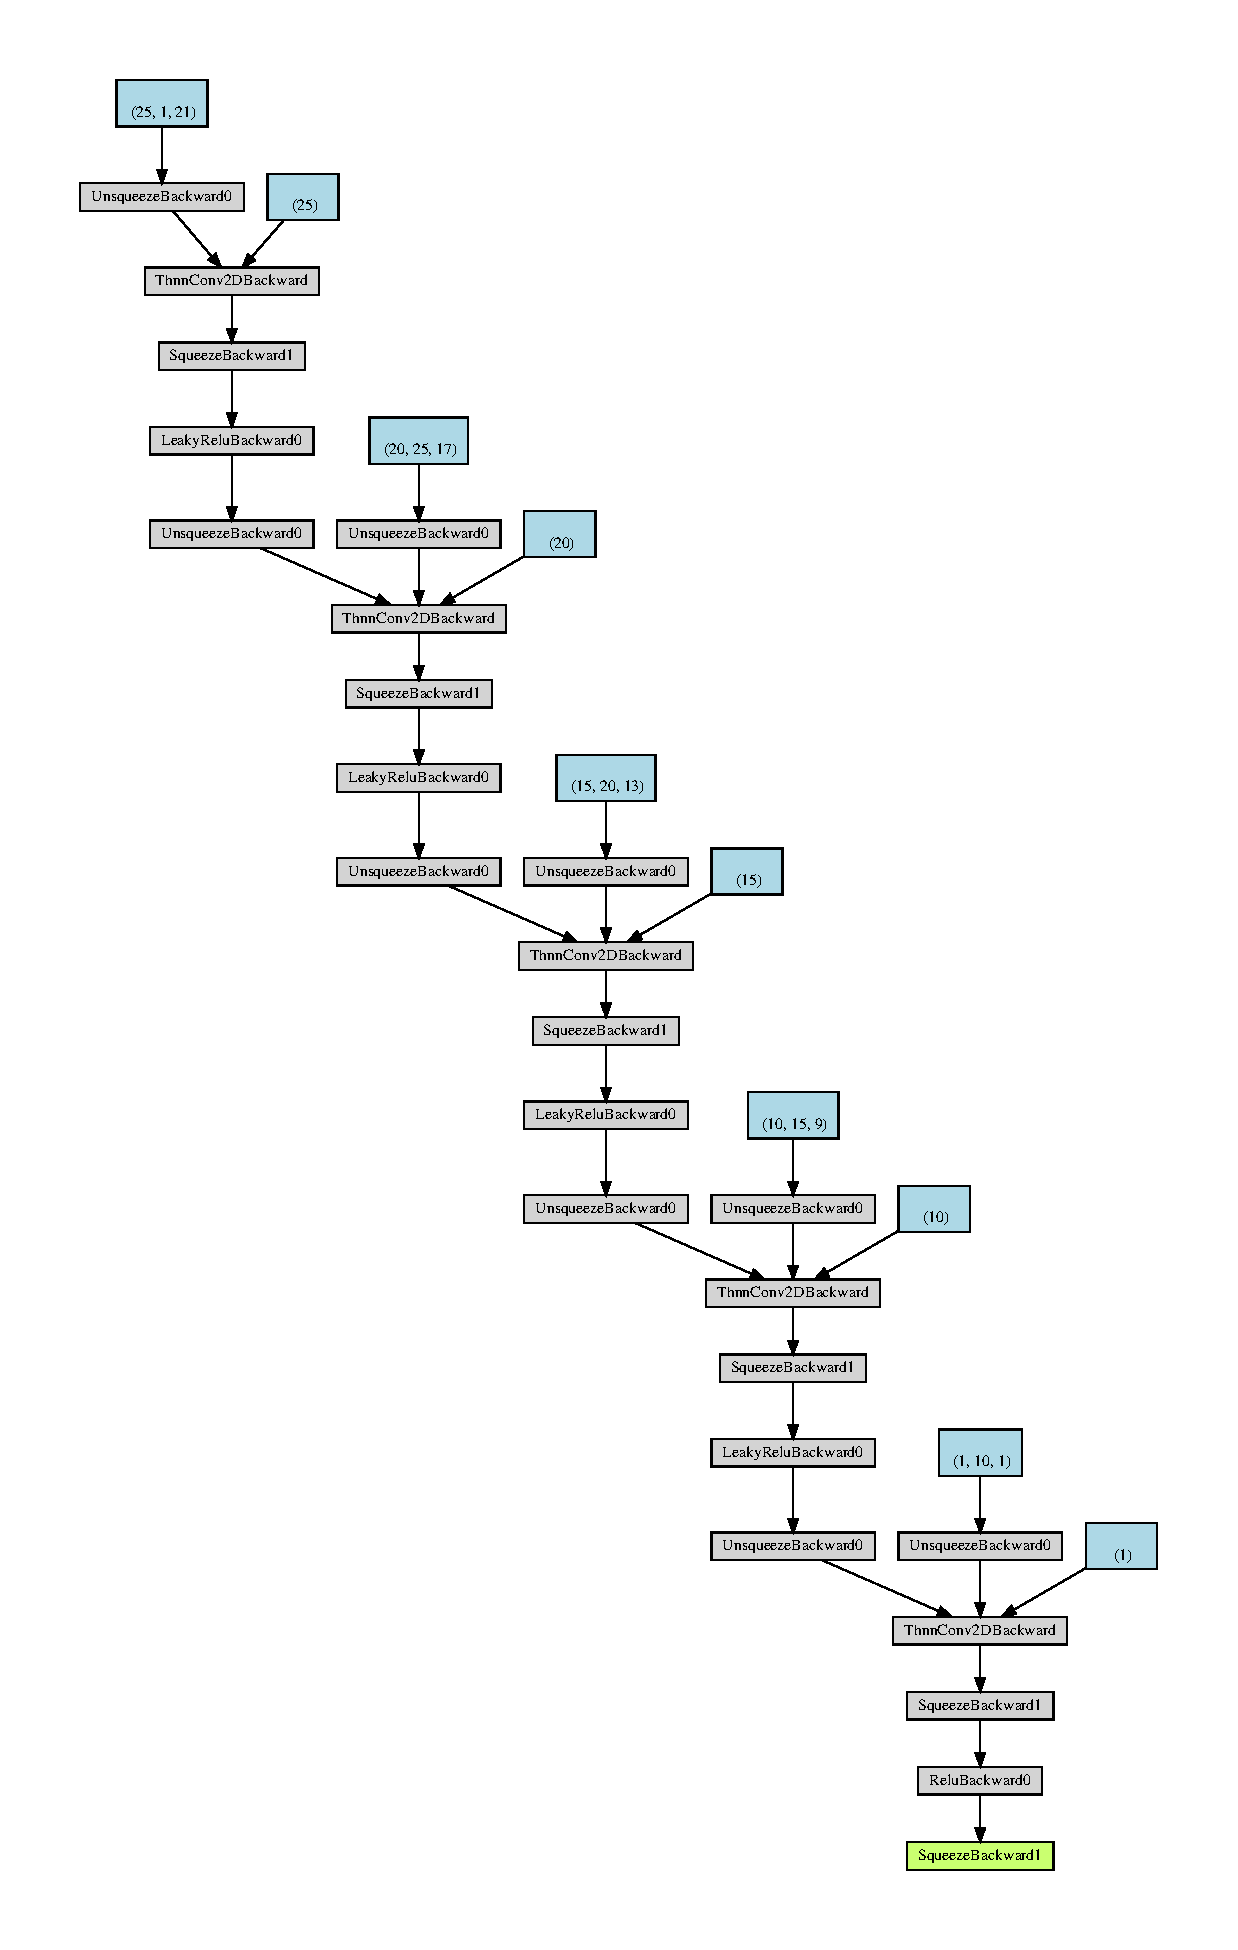
\includegraphics[width=1.0\textwidth]{img/model.pdf}
\end{figure}
\column{0.65\textwidth}
\lstinputlisting[language=Python, basicstyle=\tiny]{CNN}
\end{columns}
\end{frame}

\begin{frame}
\frametitle{Training Process}
\begin{columns}
\column{0.35\textwidth}
\begin{itemize}
    \item Train CNN by each Channel (30PMTs)
    \item $\sim$427k waveform for each Channel
    \item epoch = 36
    \item Learning rate = $0.01$
\end{itemize}
\column{0.65\textwidth}
\begin{figure}
    \centering
    \caption{Data Structure}
    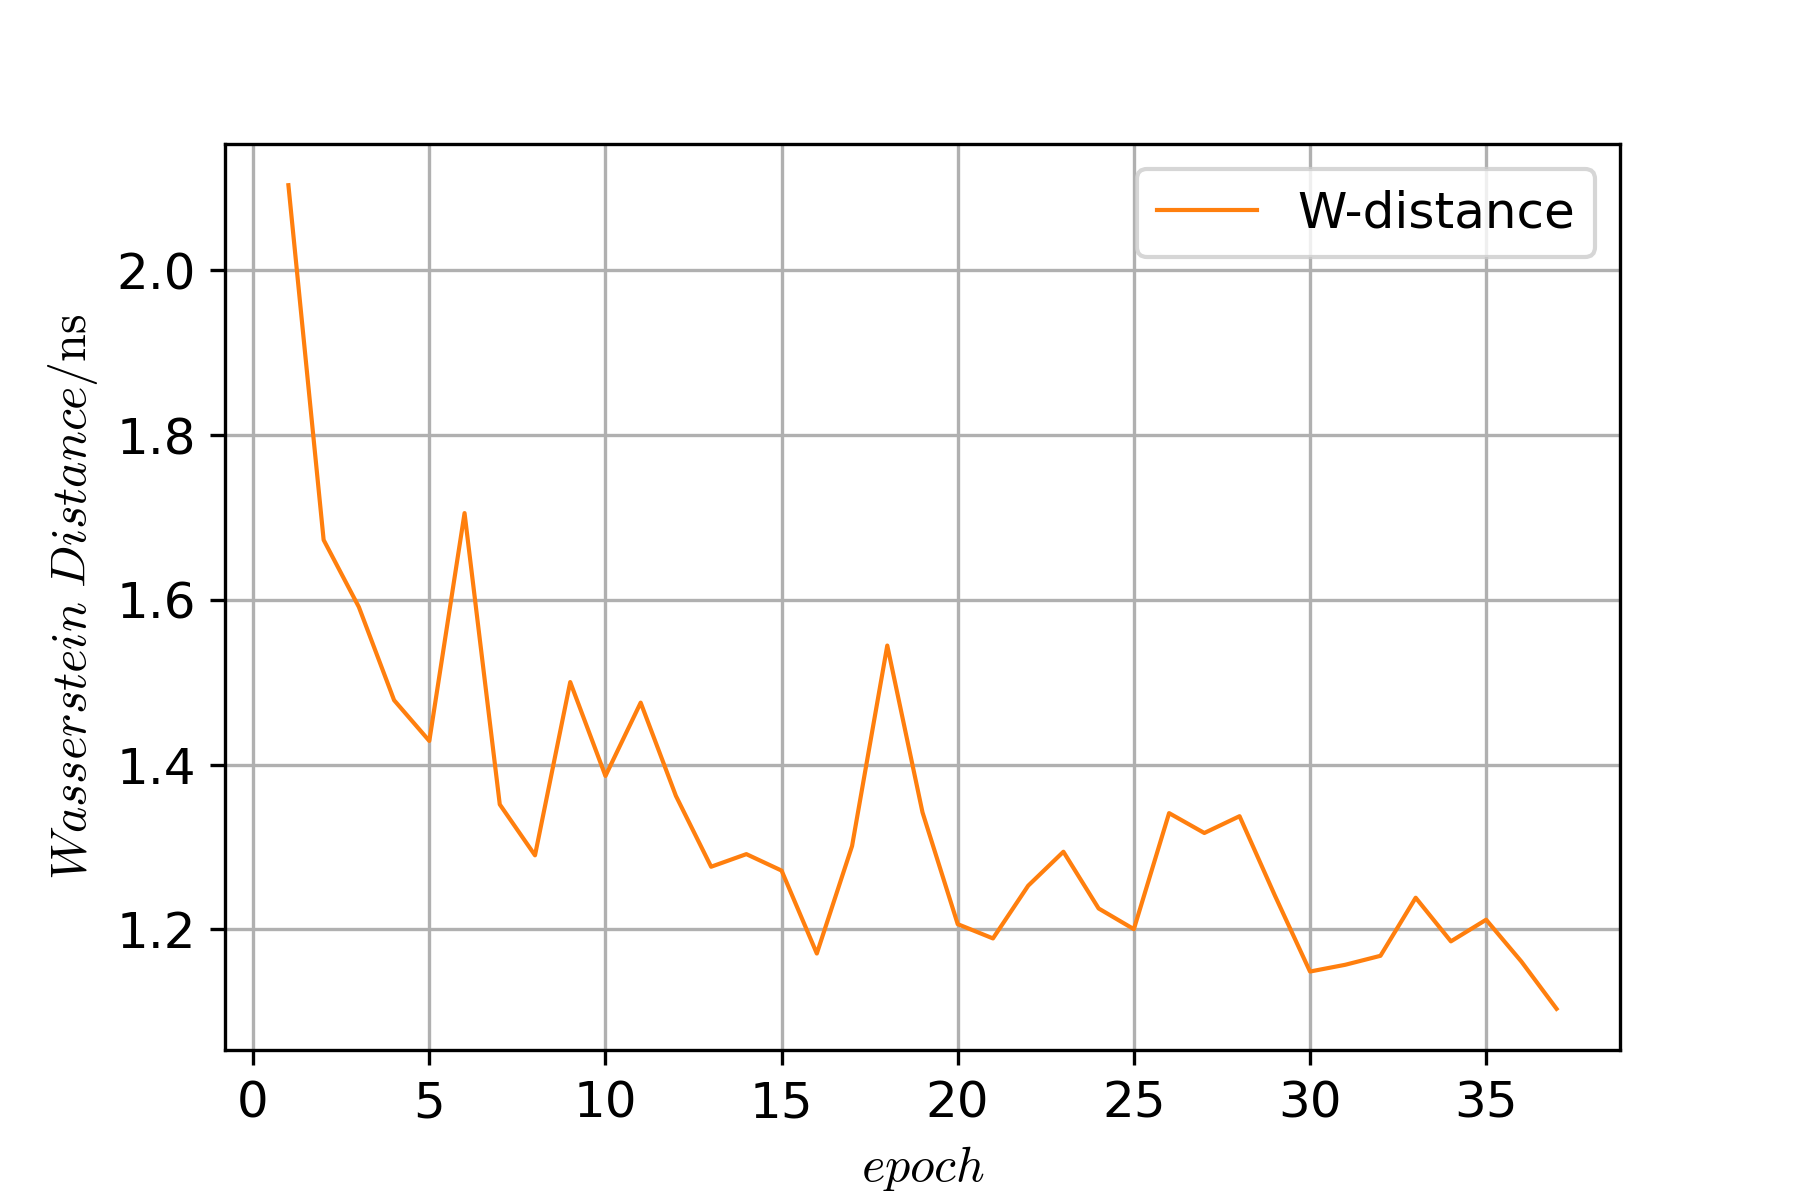
\includegraphics[width=1.0\linewidth]{img/epoch.png}
\end{figure}
\end{columns}
\end{frame}

\section{Method of Fitting}

\begin{frame}
\frametitle{Single PE Model}
\begin{figure}
    \centering
    \caption{Single PE Model}
    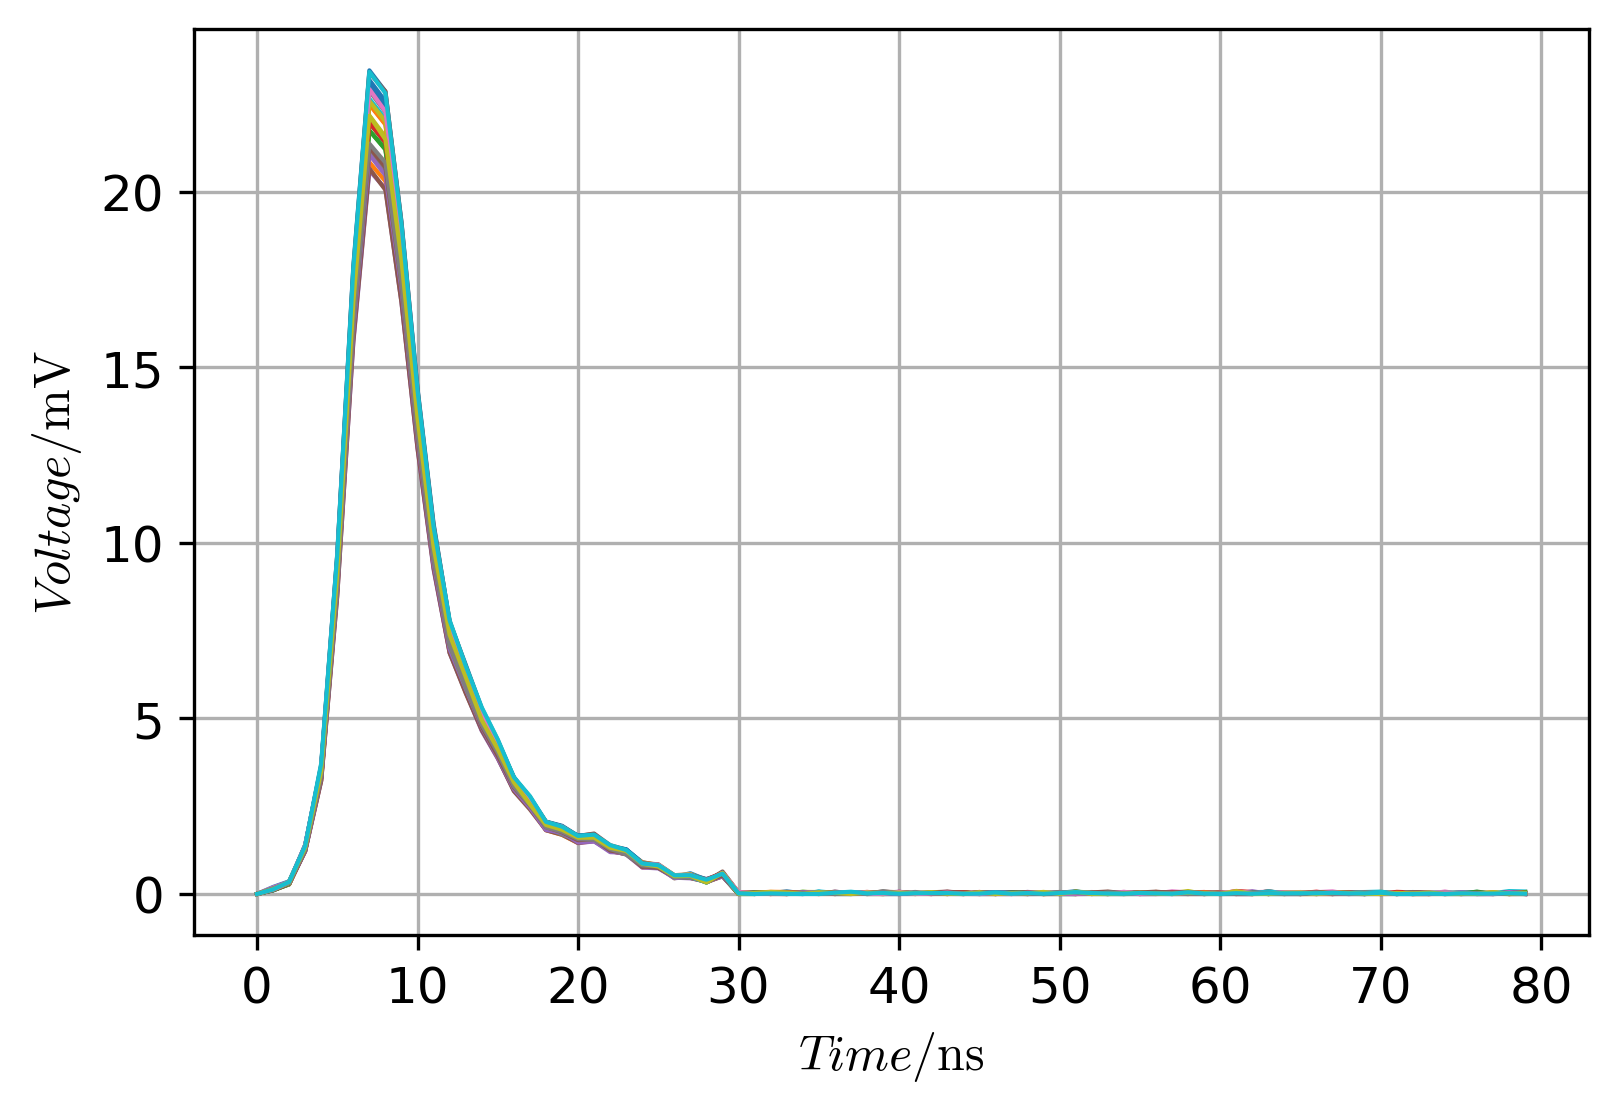
\includegraphics[width=0.9\linewidth]{img/spe.png}
\end{figure}
\end{frame}

\begin{frame}
\frametitle{Fitting Process}
\begin{itemize}
    \item Fitting parameter: Weight in each RiseTime
    \item loss is Residual sum squares of Waveform
    \item Loss = $\sum_{i}^{1029}(Wave_{recon_i}-Wave_{truth_i})^{2}$
    \item using \lstinline{scipy.optimize.fmin_l_bfgs_b}
\end{itemize}
\setlength{\belowcaptionskip}{0mm}
\begin{figure}
    \centering
    \caption{Demo}
    \includegraphics[width=0.7\linewidth]{img/demo.png}
\end{figure}
\end{frame}

% \begin{frame}
% \frametitle{Application of MCMC}
    
% \end{frame}

\section{Result}
\begin{frame}
\frametitle{Distances}
\begin{table}
    \centering
    \caption{Reconstruction Result}
    \begin{tabular}{c|c|c|c|c}
        \hline
        &  & W-dist/$\mathrm{ns}$ & P-dist/$\mathrm{1}$ & Charge-diff/$\mathrm{mV}\cdot\mathrm{ns}$ \\
        \hline
        CNN & Charge & 1.82 & - & -77.6 \\
        \hline
        CNN & PEnum & 0.79 & 0.14 & - \\
        \hline
        Fitting & Charge & 2.02 & - & -39.7 \\
        \hline
        Fitting & PEnum & 2.62 & 0.12 & - \\
        \hline
    \end{tabular}
\end{table}
\end{frame}

\begin{frame}
\frametitle{Efficiency}
\begin{table}
    \centering
    \caption{Reconstruction Efficiency}
    \begin{tabular}{c|c|c}
        \hline
        &  & Performance \\
        \hline
        CNN & Charge & 6.4s/$10^{5}$Wf \\
        \hline
        CNN & PEnum & 6.3s/$10^{5}$Wf\\
        \hline
        Fitting & Charge & 450s/$10^{5}$Wf(50cpu) \\
        \hline
        Fitting & PEnum & 560s/$10^{5}$Wf(50cpu) \\
        \hline
    \end{tabular}
\end{table}
\end{frame}

\section{Summary \& Outlook}
\begin{frame}
\frametitle{Summary \& Outlook}
\begin{itemize}
    \item We developed several representative methods to extract photon information hidden in PMT waveform
    \item These methods will improve the accuracy of following-up Event reconstruction
    \item We are working on applying and connecting these methods to Event reconstruction
\end{itemize}
\end{frame}

\begin{frame}
\frametitle{Credit}
\hspace{4mm}The ideas and methods originally come from a data contest and a summer semester course, main participants are:
\begin{itemize}
    \item Benda Xu (Tsinghua University)
    \item Yiyang Wu (Tsinghua University)
    \item Yu Xu (Forschungszentrum Jülich)
    \item $\cdots$
\end{itemize}
\end{frame}

\appendix
\section{Backup}
\begin{frame}
\frametitle{Backup}
    
\end{frame}

\end{document}